\subsection{Revving the VIPUR approach to expand rare disease diagnostics}
	\subsubsection{Preparatory steps for using the VIPUR approach}
		After the publication of VIPUR the tools, data and applications became available at the open science framework (OSF) \cite{} which were downloaded and reviewed. All applications from the Rosetta software suite (Section \ref{subsec:MM_Rosetta}) were pre-compiled without support for MPI (Section \ref{subsec:MM_MPI}) and with that not the ability to benefit from multiple CPUs. The Rosetta software suite was rebuilt with MPI support in a slurm job where the compilation could benefit from multiple CPU cores.
	\label{subsubsec:RES_Prepare}
	
	\subsubsection{VIPUR resolving system incompatibilities}
	Within the VIPUR pipeline residues were mutated to determine the effects of a structural mutation, by default missense mutations were inserted with PyMOL (Section \ref{subsec:MM_PyMOL}), an alternative method integrated within the pipeline for situations wherein PyMOL was not accessible Pyrosetta (Section \ref{subsec:MM_PyRosetta}) could be used. Neither of these programs could be built or compiled because the lack of Open graphics library (OpenGL) for PyMOL and having the incorrect C++ and C libraries for PyRosetta. To bypass both programs and still be able to introduce mutations into PDB files Modeller (Secton \ref{subsec:MM_Modeller}) was introduced and built.
	
	\begin{figure}[!ht]
		\centering
		\begin{subfigure}{0.45\textwidth}
			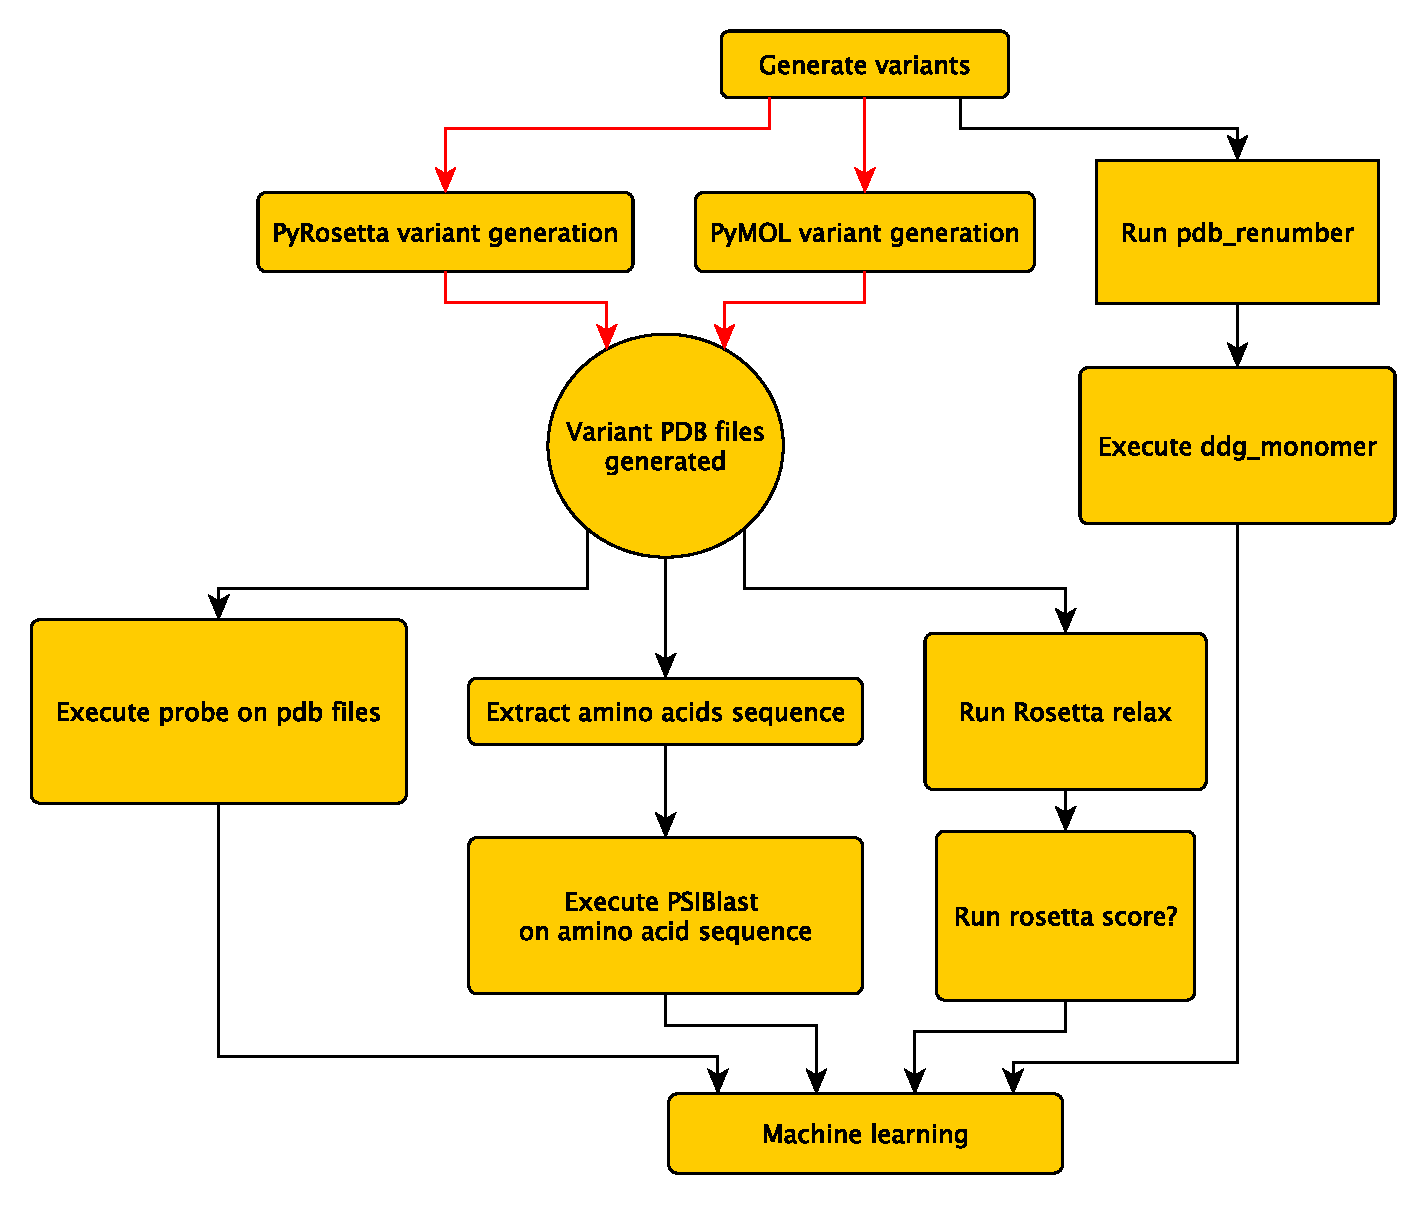
\includegraphics[width=\textwidth]{Flowcharts/VIPUR_approach.pdf}{a}
			\phantomcaption
			\label{fig:RES_VIPUR_approach}
		\end{subfigure}
		\begin{subfigure}{0.45\textwidth}
			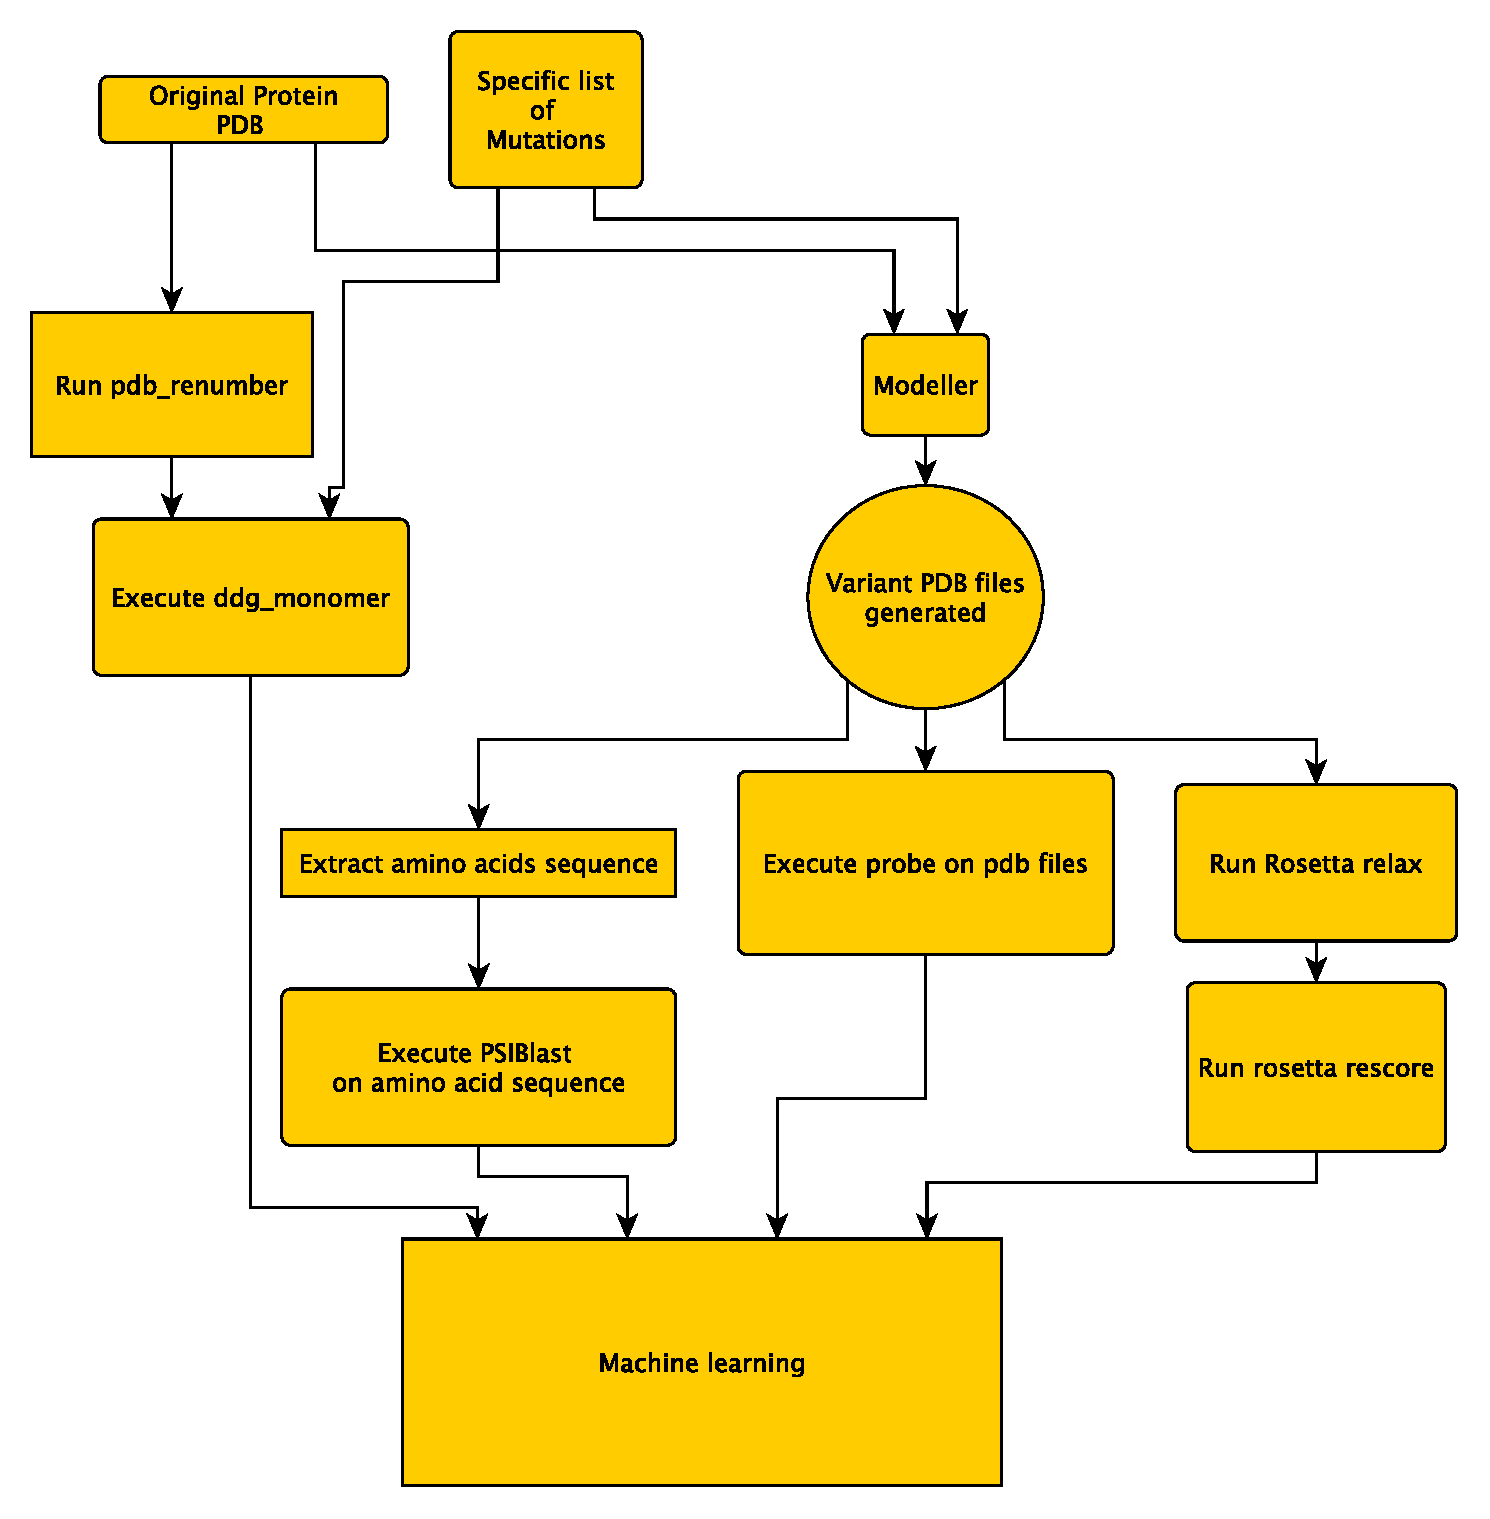
\includegraphics[width=\textwidth]{Flowcharts/Altered_VIPUR_approach.pdf}{b}
			\phantomcaption
			\label{fig:RES_Altered_VIPUR_approach}
		\end{subfigure}
		\caption[Flowcharts VIPUR pipeline and altered VIPUR pipeline]{Both flowcharts illustrate the VIPUR pipeline wherein each block is a procedure the central circle is the purpose of the mutated applications and each arrow represents the path to it. Figure \ref{fig:RES_VIPUR_approach} has red arrows that indicate that both methods were incapable to produce the mutated PDB files. Within figure \ref{fig:RES_Altered_VIPUR_approach} the alternative method is proposed wherein PyMOL and PyRosetta (Sections \ref{subsec:MM_PyMOL}, \ref{subsec:MM_PyRosetta}) is substituted by Modeller (Section \ref{subsec:MM_Modeller}) to acquire the mutated protein structures.}

		\label{fig:Flowcharts_of_old_and_altered_VIPUR}
	\end{figure}
	\label{subsubsec:RES_Incompatibility}
	\newpage
	
	\subsubsection{Expanding the VIPUR training set with data from TNFRSF1A by homology modeling and protein threading}
	Since the VTS did not have any features of TNFRSF1A (Section \ref{subsec:CD_TNFRSF1A}) the amino acid sequence was collected from Uniprot (Section \ref{subsec:MM_Uniprot}) and the protein from RCSB (Section \ref{subsec:MM_RCSB}). The structures available of TNFRSF1A were incomplete, fragments for the TNF $\alpha$ and $\beta$ active site were available and its death domain that interacts with TRADD which plays a role in apoptosis. To acquire a monomeric structure of TNFRSF1A the I-TASSER and Robetta webservices (Sections \ref{subsec:MM_I_TASSER}, \ref{subsec:MM_Robetta}) had been employed. Both had to model hte proteins with and without template to test  
	
	
	To acquire a model that might represent TNFRSF1A th the performance of both services ,that rely on two different modeling techniques (Section \ref{subsec:GD_Protein_modeling_techniques}), they had to model the whole structure with and without a template of the binding site of TNFRSF1A in were tested to form a structure based on the whole amino acid sequence, both got the would perform to make an accurate structure it wastructures of the binding site of
%	
%	\begin{figure}[!ht]
%		\centering
%		\begin{subfigure}{0.45\textwidth}
%			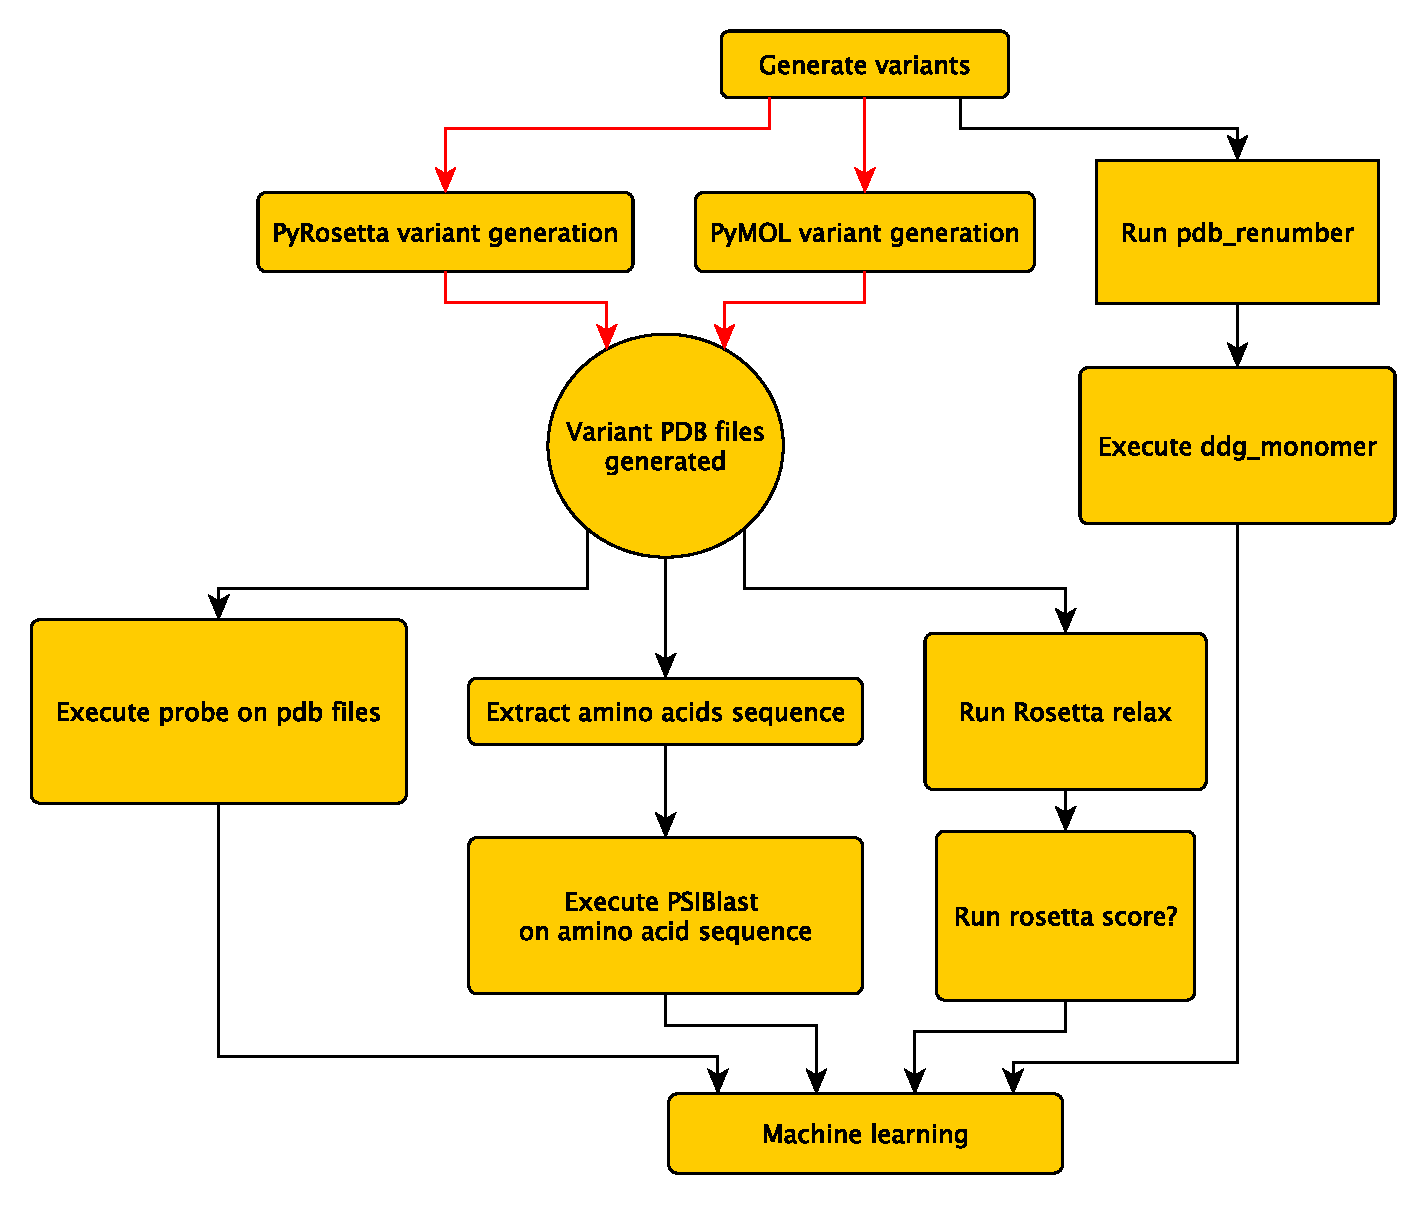
\includegraphics[width=\textwidth]{Flowcharts/VIPUR_approach.pdf}{a}
%			\phantomcaption
%			\label{fig:RES_}
%		\end{subfigure}
%		\begin{subfigure}{0.45\textwidth}
%			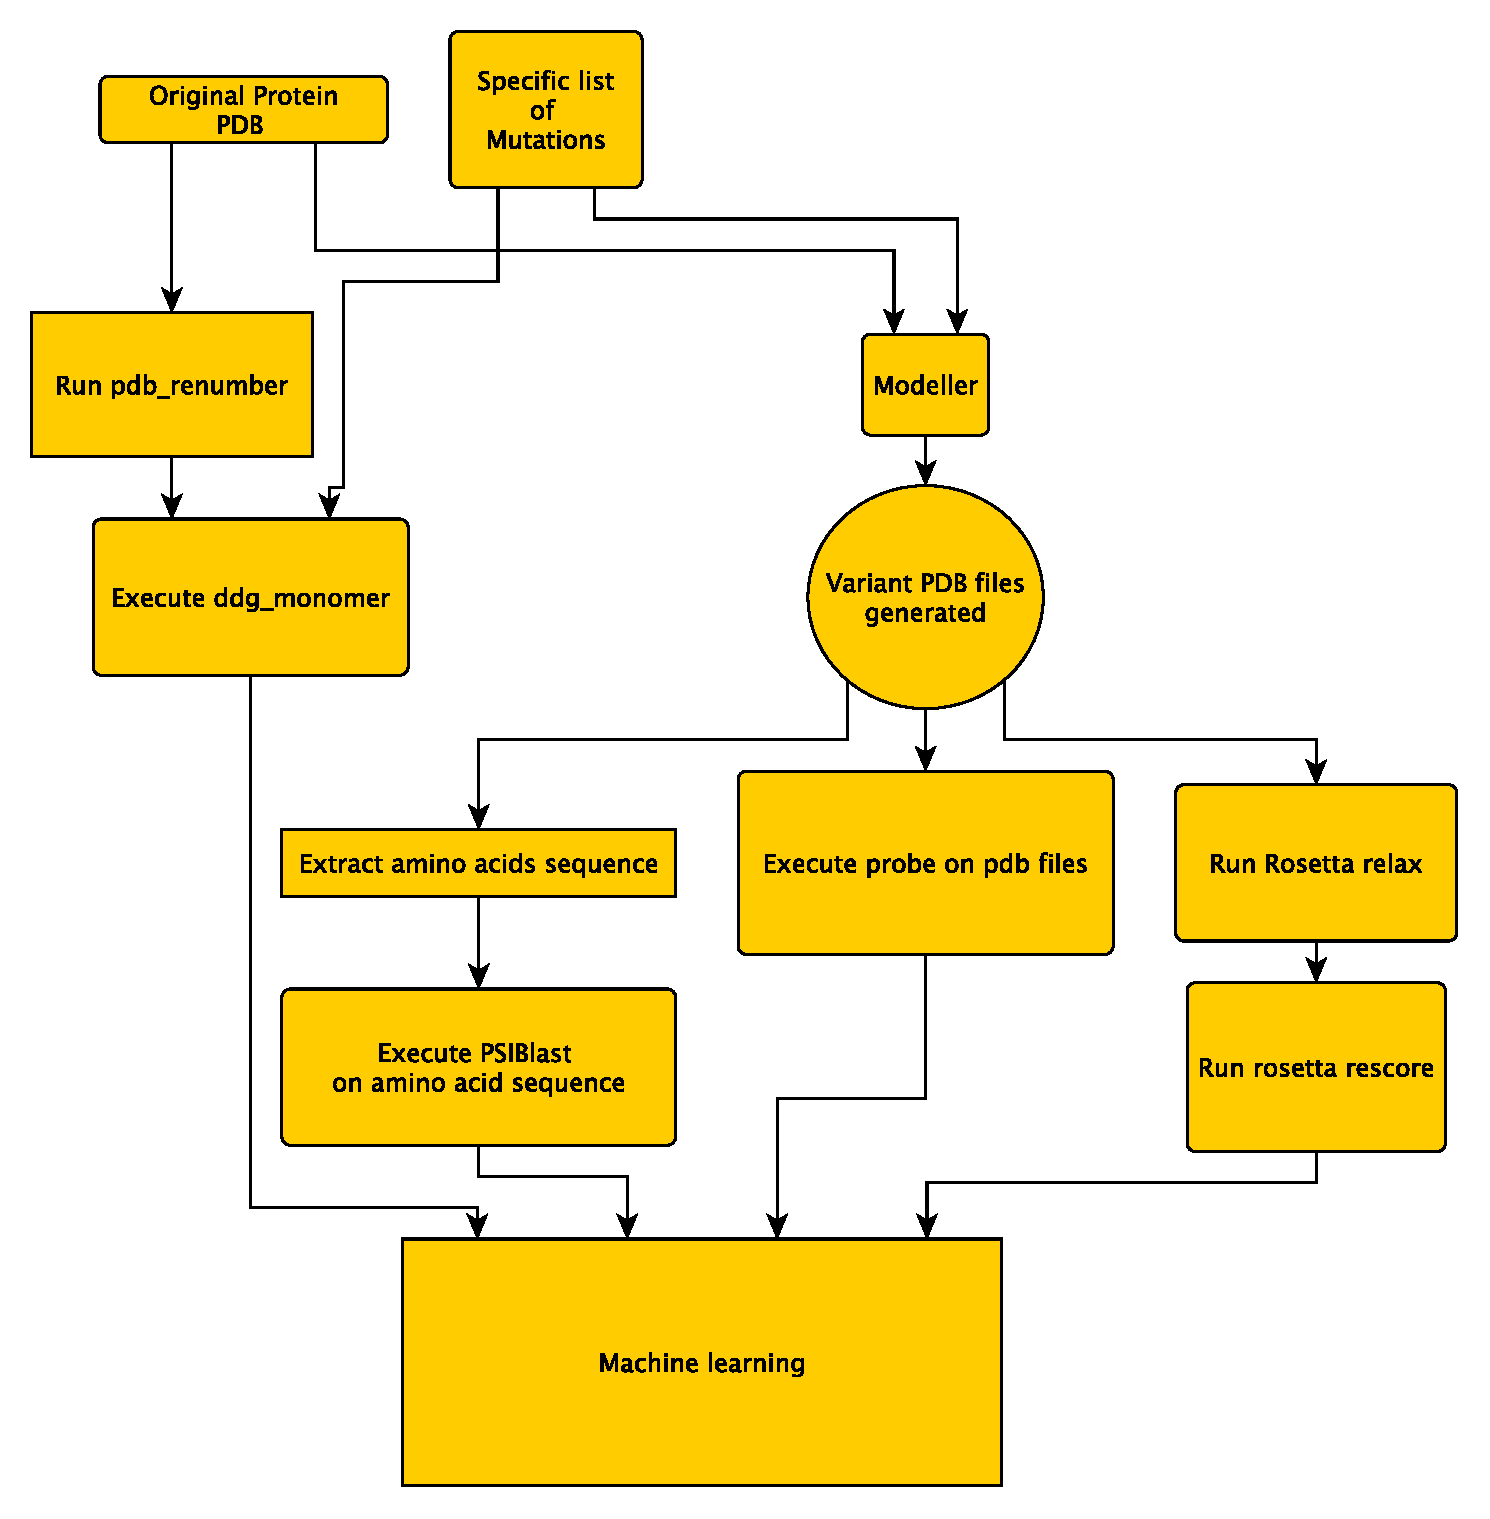
\includegraphics[width=\textwidth]{Flowcharts/Altered_VIPUR_approach.pdf}{b}
%			\phantomcaption
%			\label{fig:RES_}
%		\end{subfigure}
%		\begin{subfigure}{0.45\textwidth}
%			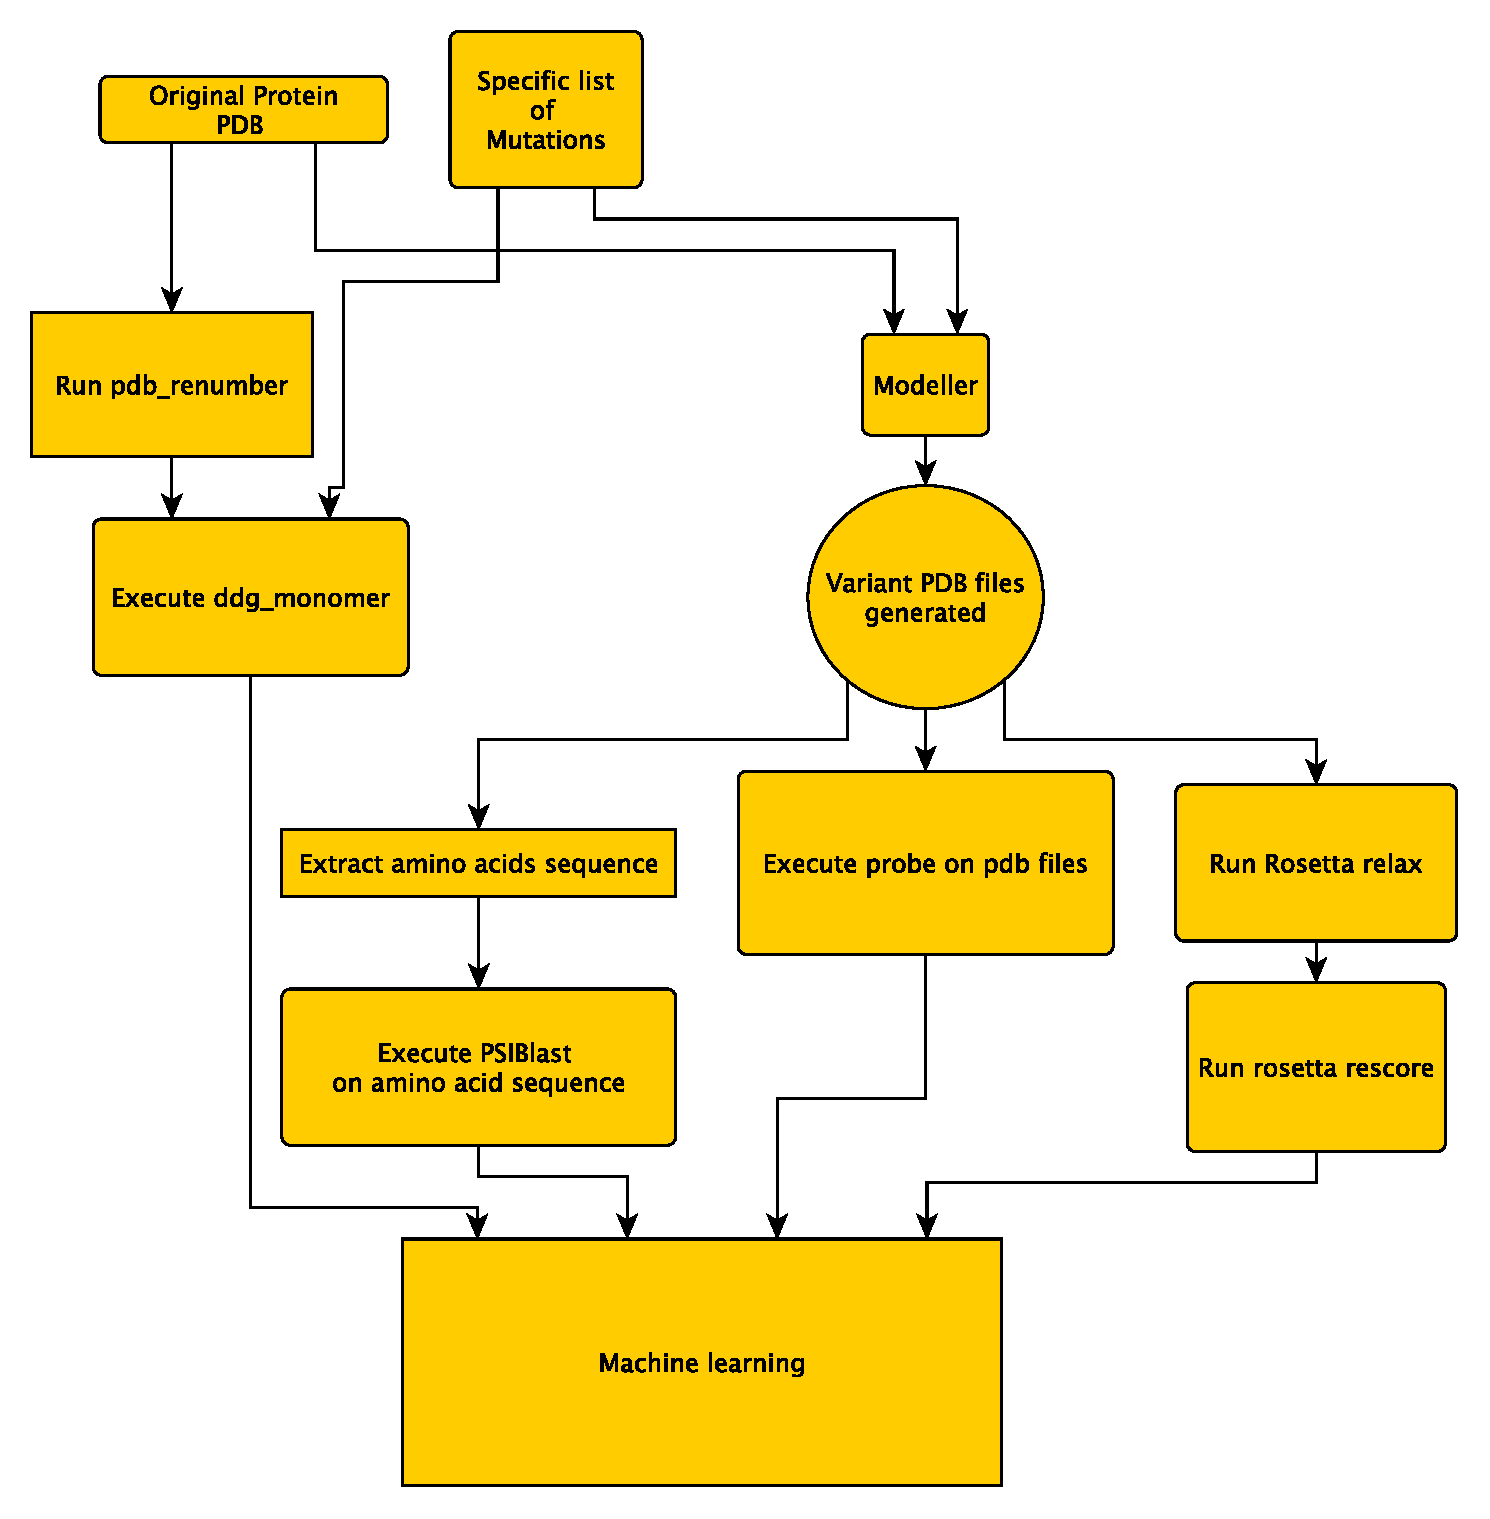
\includegraphics[width=\textwidth]{Flowcharts/Altered_VIPUR_approach.pdf}{c}
%			\phantomcaption
%			\label{fig:RES_}
%		\end{subfigure}
%		\begin{subfigure}{0.45\textwidth}
%			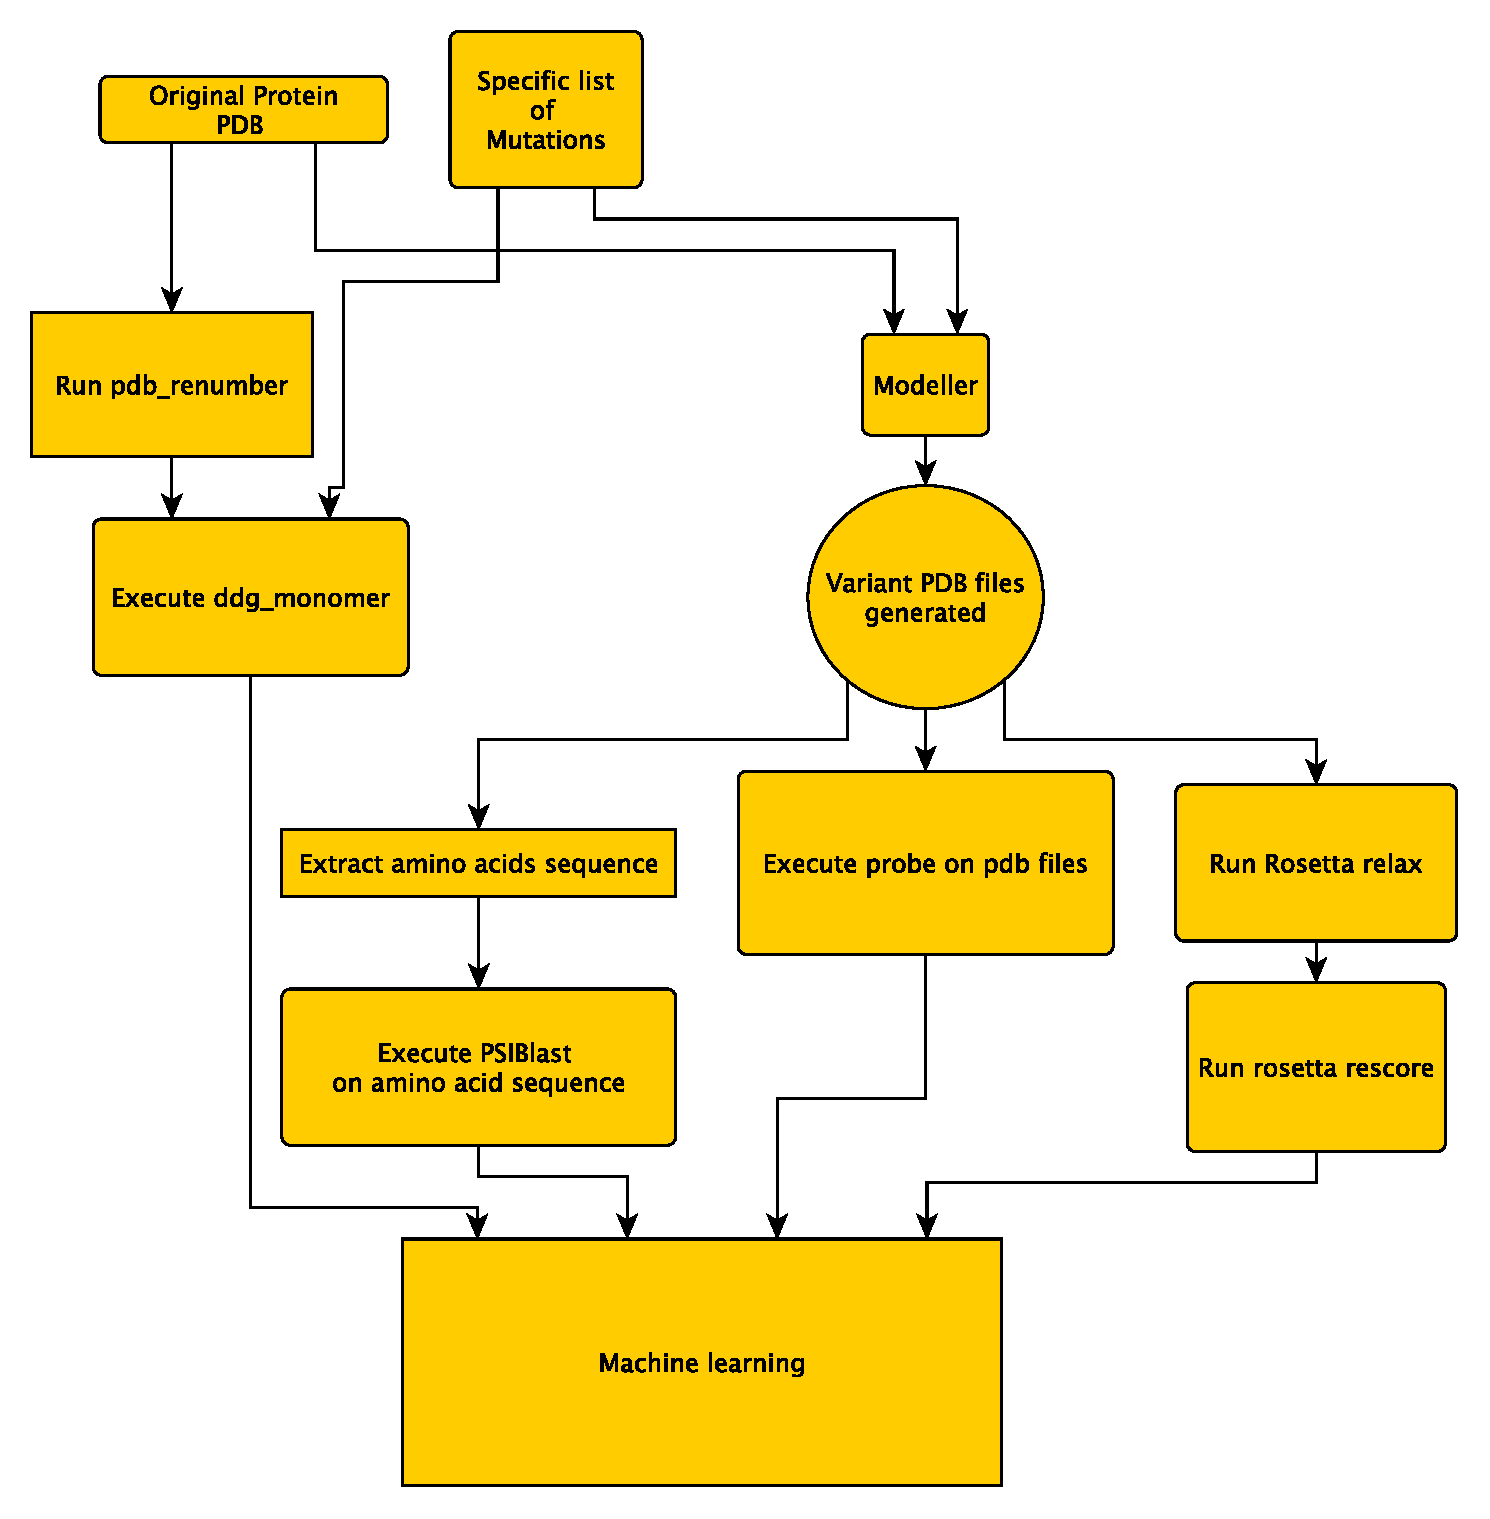
\includegraphics[width=\textwidth]{Flowcharts/Altered_VIPUR_approach.pdf}{d}
%			\phantomcaption
%			\label{fig:RES_}
%		\end{subfigure}
%		\caption[I-TASSER and Robetta models with and without templates]{}



	\label{subsubsec:RES_Expanding_Models}

%VIPUR: Variant Interpretation and Prediction Using Rosetta, Baugh
%The structures 1EXT \cite{} and 1TNR \cite{} (Sections \ref{subsec:MM_RCSB} \ref{subsec:MM_Uniprot}) that represent TNFRSF1A (Section \ref{section:Chap_Cell Death}) were incomplete and to fill in the missing pieces of the structure


%Something about that we tried to use the VTS and add our protein for information.
%\begin{table}[ht]
%	\begin{tabular}{ l | l | l | l}
%		Original residue & Position in the protein sequence & New residue & Classification\\ \hline
%		Cys & 44 & Tyr & PATHOGENIC\\
%		Thr & 44 & Pro & PATHOGENIC\\
%		Thr & 44 & Ser & PATHOGENIC\\
%	\end{tabular}
%	\caption{The format wherein mutations were filtered from the GAVIN, GenomAD and Infevers tables (Sections \ref{subsec:MM_GAVIN_data_table},  \ref{subsec:MM_GenomAD}, \ref{subsec:MM_Infevers} ) with the available classifications: Benign Pathogenic, Likely Benign, Likely Pathogenic, Population, Uncertain significance (VOUS) and Na.}
%	\label{table:Res_Filtered_Mutations}
%\end{table}
%
%\begin{table}[ht]
%	\begin{tabular}{ l | l | l | l | l}
%		Iteration number & Filename & Chain & Residue index in chain & New residue\\ \hline
%		34 & 1tnr3\_TNFA & R & 0 & TYR\\
%		34 & 1tnr3\_TNFA & T & 0 & TYR\\
%		34 & 1tnr3\_TNFA & S & 0 & TYR\\
%		35 & 1tnr3\_TNFA & R & 0 & PRO\\
%		35 & 1tnr3\_TNFA & T & 0 & PRO\\
%		35 & 1tnr3\_TNFA & S & 0 & PRO\\
%		36 & 1tnr3\_TNFA & R & 0 & SER\\
%		36 & 1tnr3\_TNFA & T & 0 & SER\\
%		36 & 1tnr3\_TNFA & S & 0 & SER\\
%	\end{tabular}
%	\caption{The format that describes the mutations that should be made by Modeller (Section \ref{subsec:MM_Modeller}). The iteration number states if a mutation must be made in a single variant or in a different protein. Filename describes the protein to which the mutations are applied. Since structures can consist of multiple chains it has to be specified together with the index starting at 0 instead of 1 and finally to which residue it will be transformed.}
%		\label{table:Res_Modeller_Mutation_Format}
%\end{table}

